\documentclass[11pt]{article}
% 커널 SVM 퀴즈 (쉬운 판: 곱하기 · 더하기만): 왜 서포트 벡터 몇 개 (α) 로 SVM 과 같은 답이 나오나, 커널은 무엇을 바꿔 끼우나
% 빌드 (이 폴더에서):  tectonic svm_kernel_quiz_solution.tex   -> 정답 (빈칸에 파란 답)
%                      tectonic svm_kernel_quiz.tex            -> 학생용 (빈칸)
% 데이터: 정수 점 8개, 덱과 같은 ‖w‖ = 1: w = (0.6, 0.8), b = -3.9, 마진 2.5, 서포트 벡터 A (4,5) · B (1,1), α = +0.2 · -0.2 (sklearn 하드 마진을 ‖w‖ 로 나눈 값, make_figs.fig_quizkid 에 assert)
% 옛 증명판 (w = u + v) 은 _이전/svm_kernel_quiz_solution_v1_증명.tex

\usepackage[a4paper,margin=2.2cm]{geometry}
\usepackage{kotex}
\usepackage{amsmath,amssymb}
\usepackage{enumitem}
\usepackage{comment}
\usepackage{xcolor}
\usepackage{fancyhdr}
\usepackage{graphicx}
\graphicspath{{../figs/}}

\ifdefined\STUDENT
  \excludecomment{answer}
  \newcommand{\blank}[2]{\underline{\hspace{#1}}}
  \newcommand{\pick}[2]{\text{(\ #1\ )}}
\else
  \specialcomment{answer}{\begingroup\par\vspace{2pt}\color{blue}\small\setlength{\parskip}{2pt}\setlength{\parindent}{0pt}\noindent\textbf{풀이.}\ }{\par\endgroup}
  \newcommand{\blank}[2]{\underline{\makebox[#1]{\color{blue}#2}}}
  \newcommand{\pick}[2]{\text{(\ {\color{blue}\textbf{#2}}\ )}}
\fi

\setlength{\headheight}{15pt}
\pagestyle{fancy}
\fancyhf{}
\fancyhead[L]{\small ML1 02-3 커널 SVM}
\fancyhead[R]{\bf 퀴즈: 서포트 벡터 몇 개로 충분한 이유\ifdefined\STUDENT\else\ \ (정답)\fi}
\fancyfoot[C]{\thepage}
\setlength{\parskip}{0.06in}
\setlength{\parindent}{0pt}

\newcounter{q}
\newcommand{\q}[1]{\par\vspace{10pt}\refstepcounter{q}{\large\bf Q\theq.}\ {\bf #1}\par\vspace{2pt}}
\newenvironment{parts}{\begin{enumerate}[label=(\alph*),leftmargin=2.2em,itemsep=7pt,topsep=2pt]}{\end{enumerate}}
\newcommand{\key}[1]{\par\vspace{6pt}\noindent\fbox{\parbox{\dimexpr\linewidth-2\fboxsep-2\fboxrule}{#1}}\par}

\begin{document}

\key{{\bf 이 퀴즈는 곱하기와 더하기만 쓴다.}\\[3pt]
{\bf 점곱}: 두 점의 같은 자리끼리 곱해서 더한다. \quad $(a,\ b)\cdot(c,\ d) = a\times c + b\times d$\\[2pt]
예: \ $(2,\ 2)\cdot(4,\ 1) = 2\times4 + 2\times1 = 10$}

%%%%%%%%%%%%%%%%%%%%%%%%%%%%%%%%%%%%%%%%%%%%%%%%%%%%%%%%%%%%%%%%%%%%
\q{경계선의 화살표 $\mathbf{w}$ 를 점으로 만들기}
\begin{center}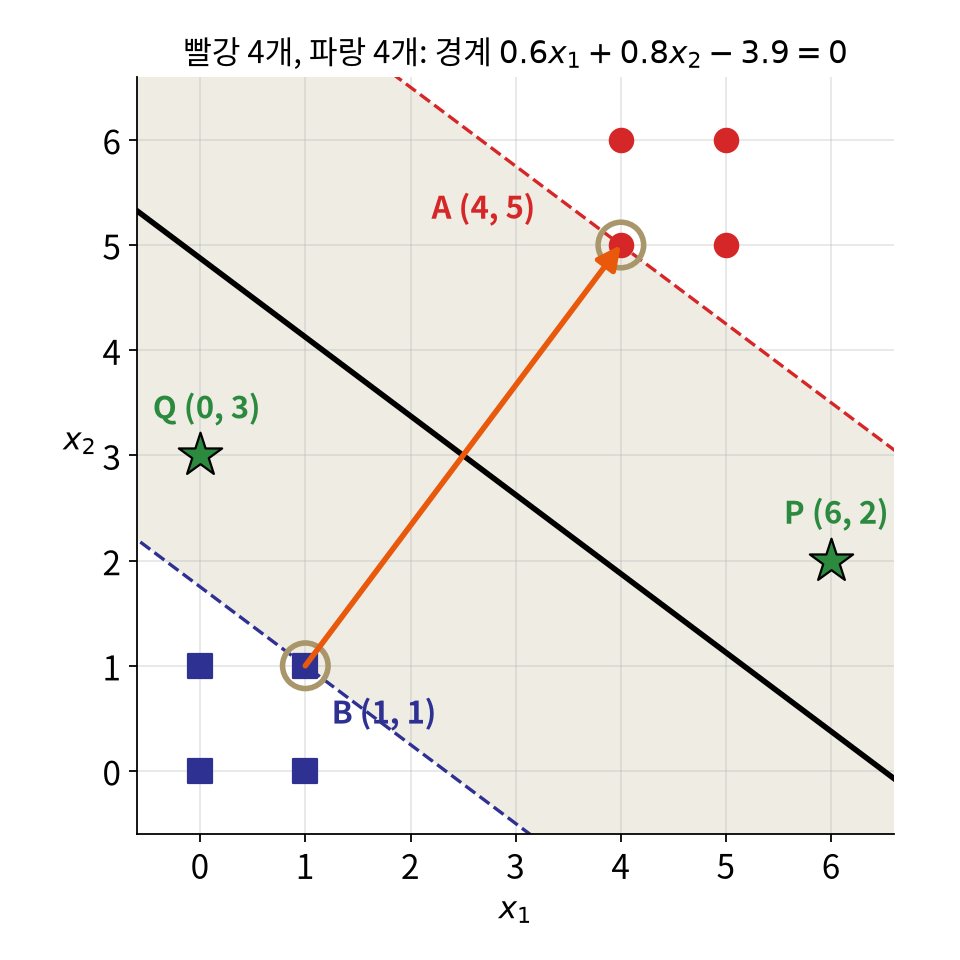
\includegraphics[width=0.5\linewidth]{kn_quizkid.png}\end{center}
\vspace{-6pt}
SVM 이 찾은 경계선: \ $\mathbf{w}\cdot\mathbf{x} + b = 0$, \ $\mathbf{w} = (0.6,\ 0.8)$, \ $b = -3.9$. \ (덱과 같은 약속: $\lVert\mathbf{w}\rVert = 1$ 이라 $f = \mathbf{w}\cdot\mathbf{x} + b$ = 경계까지 거리)\\
점선(길의 가장자리) 위에 있는 \textcolor{red}{A $(4, 5)$} 와 \textcolor{blue}{B $(1, 1)$} 이 서포트 벡터다.
\begin{parts}
\item $\mathbf{w}$ 의 길이가 1 인지 확인: \ $0.6\times0.6 + 0.8\times0.8 = \blank{0.9cm}{0.36} + \blank{0.9cm}{0.64} = \blank{0.9cm}{1}$
\item 주황 화살표는 B 에서 A 로 간다. \quad A $-$ B $= (4 - 1,\ 5 - 1) = (\,\blank{0.8cm}{3},\ \blank{0.8cm}{4}\,)$\\[2pt]
$0.2\times(3,\ 4) = (\,\blank{0.8cm}{0.6},\ \blank{0.8cm}{0.8}\,)$ \quad $\to$ $\mathbf{w}$ 와 \pick{같다 / 다르다}{같다}
\item 그래서 \quad $\mathbf{w} = (+0.2)\times\text{A} + (-0.2)\times\text{B}$.\\
이 $+0.2$, $-0.2$ 가 $\alpha$ (그 점을 얼마나 쓰는지) 다. 나머지 6개 점의 $\alpha$ 는 \blank{0.8cm}{0}.
\item 멀리 있는 빨강 $(5, 6)$ 을 지우면 경계선은 \pick{바뀐다 / 안 바뀐다}{안 바뀐다} \ $\to$ 그래서 그 점은 안 써도 된다 ($\alpha = 0$).
\end{parts}
\begin{answer}
경계선은 가장 가까운 점(서포트 벡터)만 보고 정해진다. 그래서 $\mathbf{w}$ 를 만들 때도 서포트 벡터만 쓴다.
\end{answer}

%%%%%%%%%%%%%%%%%%%%%%%%%%%%%%%%%%%%%%%%%%%%%%%%%%%%%%%%%%%%%%%%%%%%
\clearpage
\q{한 번에 계산 vs 서포트 벡터로 나눠 계산}
새 점은 $f = \mathbf{w}\cdot\mathbf{x} + b$ 의 부호로 나눈다 ($+$ 면 빨강, $-$ 면 파랑). $\lVert\mathbf{w}\rVert = 1$ 이라 $f$ 의 크기는 경계까지 거리다.\\
$\mathbf{w}\cdot\mathbf{x}$ 를 두 가지 방법으로 계산해 보자. \ ($\mathbf{w} = (0.6,\ 0.8)$, \ $b = -3.9$, \ $\alpha_\text{A} = +0.2$, \ $\alpha_\text{B} = -0.2$)
\begin{parts}
\item 새 점 \textcolor{green!45!black}{P $(6, 2)$}
\begin{itemize}[leftmargin=1.5em,itemsep=4pt]
\item 한 번에: \quad $\mathbf{w}\cdot\text{P} = 0.6\times6 + 0.8\times2 = \blank{0.9cm}{3.6} + \blank{0.9cm}{1.6} = \blank{0.9cm}{5.2}$
\item 나눠서: \quad $\text{A}\cdot\text{P} = 4\times6 + 5\times2 = \blank{0.9cm}{34}$, \quad $\text{B}\cdot\text{P} = 1\times6 + 1\times2 = \blank{0.9cm}{8}$\\[3pt]
\hspace*{4.6em}$0.2\times34 \ - \ 0.2\times8 = \blank{0.9cm}{6.8} - \blank{0.9cm}{1.6} = \blank{0.9cm}{5.2}$
\item 두 방법은 \pick{같다 / 다르다}{같다}. \quad $f = 5.2 - 3.9 = \blank{0.9cm}{1.3}$ \ $\to$ \pick{빨강 / 파랑}{빨강}, 경계에서 1.3 떨어져 있다.
\end{itemize}
\item 새 점 \textcolor{green!45!black}{Q $(0, 3)$}
\begin{itemize}[leftmargin=1.5em,itemsep=4pt]
\item 한 번에: \quad $\mathbf{w}\cdot\text{Q} = 0.6\times0 + 0.8\times3 = \blank{0.9cm}{2.4}$
\item 나눠서: \quad $\text{A}\cdot\text{Q} = \blank{0.9cm}{15}$, \quad $\text{B}\cdot\text{Q} = \blank{0.9cm}{3}$, \quad $0.2\times15 - 0.2\times3 = \blank{0.9cm}{2.4}$
\item $f = 2.4 - 3.9 = \blank{0.9cm}{$-1.5$}$ \ $\to$ \pick{빨강 / 파랑}{파랑}
\end{itemize}
\item 그러니 $\mathbf{w}$ 를 몰라도, 서포트 벡터 \blank{0.8cm}{2} 개와 새 점의 점곱에 $\alpha$ 를 곱해 더하면 같은 답이 나온다.
\end{parts}
\key{{\bf 왜 같을까?} \ $\mathbf{w}$ 가 원래 $0.2\times(\text{A} - \text{B})$ 이니까, $\mathbf{w}\cdot\text{P} = 0.2\times\text{A}\cdot\text{P} - 0.2\times\text{B}\cdot\text{P}$.\\
1000원을 500원 동전 2개로 세어도 1000원인 것처럼, 같은 화살표를 다르게 적은 것뿐이다.}

%%%%%%%%%%%%%%%%%%%%%%%%%%%%%%%%%%%%%%%%%%%%%%%%%%%%%%%%%%%%%%%%%%%%
\clearpage
\q{서포트 벡터가 3개면?}
\begin{center}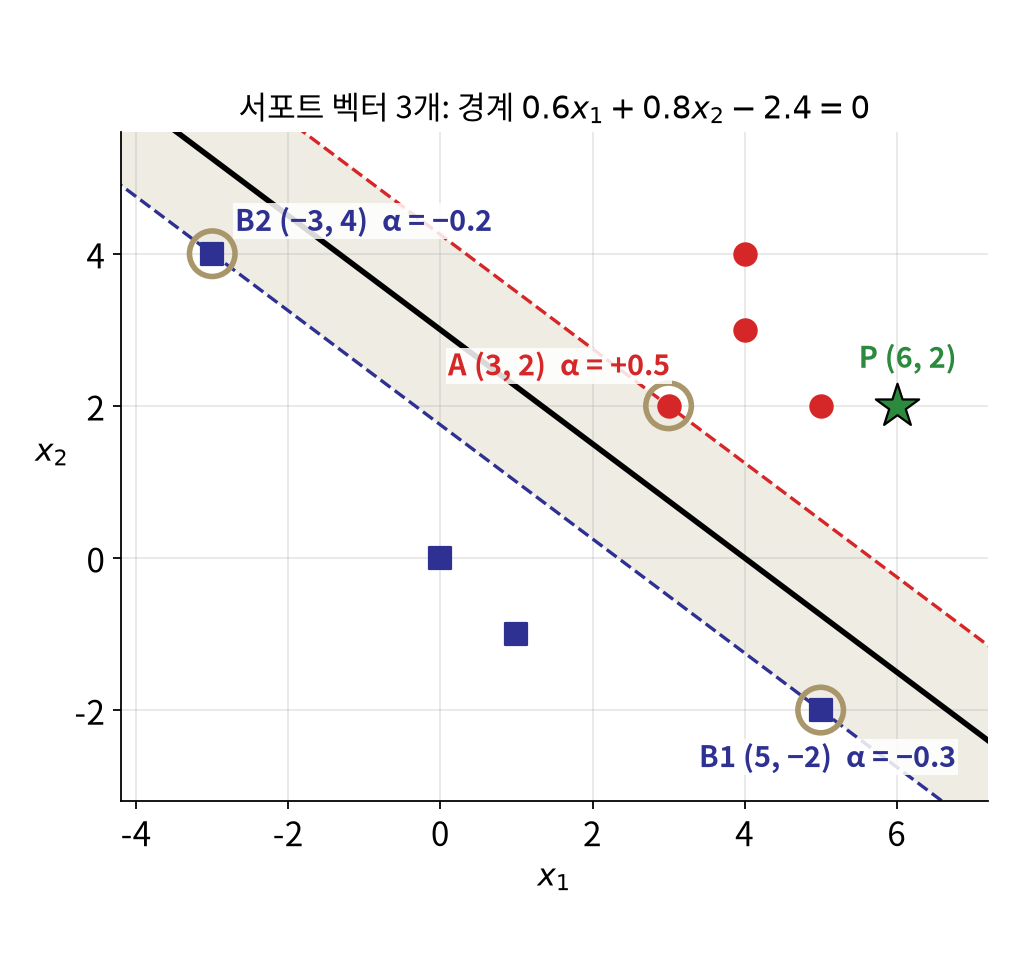
\includegraphics[width=0.5\linewidth]{kn_quizkid3.png}\end{center}
\vspace{-6pt}
점을 바꿨더니 $\mathbf{w}$ 는 Q1 과 같은 $(0.6,\ 0.8)$, \ $b = -2.4$, 마진 1, 서포트 벡터는 3개가 되었다.\\
\textcolor{red}{A $(3, 2)$: $\alpha = +0.5$}, \quad \textcolor{blue}{B1 $(5, -2)$: $\alpha = -0.3$}, \quad \textcolor{blue}{B2 $(-3, 4)$: $\alpha = -0.2$}
\begin{parts}
\item $\mathbf{w} = 0.5\times\text{A} - 0.3\times\text{B1} - 0.2\times\text{B2}$ 를 자리마다 계산하라.
\begin{itemize}[leftmargin=1.5em,itemsep=3pt]
\item 첫째 자리: \ $0.5\times3 - 0.3\times5 - 0.2\times(-3) = \blank{0.8cm}{1.5} - \blank{0.8cm}{1.5} + \blank{0.8cm}{0.6} = \blank{0.8cm}{0.6}$
\item 둘째 자리: \ $0.5\times2 - 0.3\times(-2) - 0.2\times4 = \blank{0.8cm}{1.0} + \blank{0.8cm}{0.6} - \blank{0.8cm}{0.8} = \blank{0.8cm}{0.8}$
\item $\mathbf{w}$ 와 \pick{같다 / 다르다}{같다}
\end{itemize}
\item 미는 힘: \ 빨강 $0.5$ \ = \ 파랑 $\blank{0.8cm}{0.3} + \blank{0.8cm}{0.2}$ \quad $\to$ 양쪽 힘이 \pick{같다 / 다르다}{같다}\\[2pt]
{\small 왜 같아야 할까? \ 한쪽이 더 세게 밀면 경계가 다른 쪽으로 밀려 간다. 같아야 경계가 멈춘다. 그래서 $\alpha$ 를 부호까지 다 더하면 $0.5 - 0.3 - 0.2 = \blank{0.8cm}{0}$ (늘 0).}
\item 파랑 둘의 힘은 왜 다를까? \ 경계를 따라 재면 A 에서 B1 은 4, B2 는 6 떨어져 있다.\\[2pt]
$0.3\times4 = \blank{0.8cm}{1.2}$, \quad $0.2\times6 = \blank{0.8cm}{1.2}$ \quad $\to$ 시소처럼 (힘 $\times$ 거리) 가 같다. A 에 \pick{가까운 / 먼}{가까운} 점이 더 세게 민다.\\[2pt]
{\small 시소가 맞아야 경계가 \textbf{돌지 않는다}. 그래서 (a) 의 합 $0.5\times\text{A} - 0.3\times\text{B1} - 0.2\times\text{B2}$ 는 옆으로 삐져나가지 않고 경계에 수직인 $\mathbf{w}$ 방향과 딱 맞는다. \ (b) 안 밀려 감 $+$ (c) 안 돎 $=$ $\mathbf{w}$ = ($\alpha \times$ 점) 의 합.}
\item 새 점 \textcolor{green!45!black}{P $(6, 2)$} 를 서포트 벡터 3개로 나눠 계산:
\begin{itemize}[leftmargin=1.5em,itemsep=3pt]
\item $\text{A}\cdot\text{P} = 3\times6 + 2\times2 = \blank{0.8cm}{22}$, \quad $\text{B1}\cdot\text{P} = \blank{0.8cm}{26}$, \quad $\text{B2}\cdot\text{P} = (-3)\times6 + 4\times2 = \blank{0.8cm}{$-10$}$
\item $0.5\times(\text{A}\cdot\text{P}) \ - \ 0.3\times(\text{B1}\cdot\text{P}) \ - \ 0.2\times(\text{B2}\cdot\text{P}) = \blank{0.8cm}{11} - \blank{0.8cm}{7.8} + \blank{0.8cm}{2} = \blank{0.8cm}{5.2}$
\item 한 번에: \ $\mathbf{w}\cdot\text{P} = 0.6\times6 + 0.8\times2 = 5.2$ 와 \pick{같다 / 다르다}{같다}. \quad $f = 5.2 - 2.4 = \blank{0.8cm}{2.8}$ $\to$ \pick{빨강 / 파랑}{빨강}
\end{itemize}
\item 서포트 벡터가 2개면 2줄, 3개면 \blank{0.8cm}{3} 줄을 더한다. 답은 \pick{같다 / 다르다}{같다}.
\end{parts}
\key{{\bf 몇 개든 규칙은 하나}: \ $\mathbf{w}$ = 서포트 벡터마다 ($\alpha \times$ 점) 을 다 더한 것. \ 분류 = 서포트 벡터마다 ($\alpha \times$ 점곱) 을 다 더하고 $b$.}

%%%%%%%%%%%%%%%%%%%%%%%%%%%%%%%%%%%%%%%%%%%%%%%%%%%%%%%%%%%%%%%%%%%%
\clearpage
\q{점곱 자리에 다른 계산을 끼우면: 커널}
Q2 · Q3 의 "나눠서" 계산에는 점끼리의 점곱만 나온다. 그 자리를 \textbf{점곱의 제곱}으로 바꿔 보자.\\
두 점 \ $\mathbf{x} = (1,\ 2)$, \ $\mathbf{x}' = (3,\ 1)$.
\begin{parts}
\item 점곱 \ $\mathbf{x}\cdot\mathbf{x}' = 1\times3 + 2\times1 = \blank{0.9cm}{5}$, \qquad 그 값을 제곱하면 \ $\blank{0.9cm}{25}$
\item 이번엔 점을 숫자 4개로 늘린다: \quad $(x_1,\ x_2) \ \to\ (x_1\times x_1,\ \ x_1\times x_2,\ \ x_2\times x_1,\ \ x_2\times x_2)$
\begin{itemize}[leftmargin=1.5em,itemsep=4pt]
\item $(1,\ 2) \ \to\ (1,\ 2,\ 2,\ 4)$
\item $(3,\ 1) \ \to\ (\,\blank{0.7cm}{9},\ \blank{0.7cm}{3},\ \blank{0.7cm}{3},\ \blank{0.7cm}{1}\,)$
\item 늘린 4개끼리 점곱: \ $1\times9 + 2\times3 + 2\times3 + 4\times1 = \blank{0.7cm}{9} + \blank{0.7cm}{6} + \blank{0.7cm}{6} + \blank{0.7cm}{4} = \blank{0.9cm}{25}$
\end{itemize}
\item (a) 와 (b) 는 \pick{같다 / 다르다}{같다}.\\
$\to$ 숫자를 4개로 늘려서 점곱한 값을, 늘리지 않고 원래 점곱 하나를 \blank{1.2cm}{제곱} 해서 얻었다.
\item 그래서 Q2 의 "나눠서" 계산에서 점곱 자리를 \textbf{점곱의 제곱}으로 바꾸면,\\
점을 숫자 \blank{0.8cm}{4} 개로 늘린 뒤 SVM 을 한 것과 같다. 이때 점을 실제로 \pick{늘린다 / 안 늘린다}{안 늘린다}.\\
이렇게 끼우는 계산 $K(\mathbf{x}, \mathbf{x}') = (\mathbf{x}\cdot\mathbf{x}')^2$ 을 \textbf{커널}이라고 부른다.
\end{parts}
\key{{\bf 한 줄 정리}\\[2pt]
$\mathbf{w}$ = 서포트 벡터 몇 개를 더하고 뺀 것 \ $\to$ \ 분류 = 서포트 벡터와의 점곱을 더하고 뺀 것 \ $\to$ \ 그 점곱 자리에 $K$ 를 끼우면 커널 SVM}
\begin{answer}
(b) $3\times3 = 9$, \ $3\times1 = 3$, \ $1\times3 = 3$, \ $1\times1 = 1$.
\end{answer}

\end{document}
